\chapter{Quickly Searching Explicit Expensive Graphs}
\label{chap:inflate}

In order for an articulated robot to perform manipulation tasks
in changing, unstructured environments,
it must be able to quickly solve motion planning queries in its
configuration space.
While there are many types of approaches for such queries
which we discuss in Section~\ref{sec:related-work},
one of the most common are graph search algorithms.
In this chapter,
we discuss the efficiency tradeoffs induced by formulating
the articulated motion planning problem as best-first search,
propose a general planning framework which accounts for these tradeoffs,
and examine some empirical results.

\paragraph{Two Notions of Efficiency.}

Throughout this chapter,
we reference two different types of efficiency
with regard to robotic tasks.
First, once a planner has computed a solution path or trajectory,
there is the cost incurred while executing that trajectory.
This is the traditional cost optimized for by planners.
Second, there is the cost incurred from actually computing the solution
itself.

This dichotomy of effort is, of course, not new.
From Winston's \emph{Articifial Intelligence} \cite{winston1977ai},
\begin{quote}
   ``Properly speaking, the problem of determining a good path is a search
   problem in which two kinds of effort are involved:
   \begin{itemize}
   \item First, there is the effort expended in \emph{finding} either
      some path or the best path.
   \item And, second, there is the effor actually expended in
      \emph{traversing} the network.''
   \end{itemize}
\end{quote}

For the application of manipulation planning for articulated robots,
in paricular,
the costs associated with these two components tend to be of comparable
magnitude.
For example,
when time is used as an efficency metric,
both planning and execution times for household applications
tend to be on the order of 1-2 seconds.
Alternatively, given
modern computational and actuator technologies for human-scale problems,
both planning and execution tend to consume similar amounts of energy.
Therefore,
the manipulation problem demands that
(a) the cost of plans and
(b) the cost of planning both be considered.

\paragraph{General Problem Characterization.}

We are motivated to solve motion planning problems for articulated robots.
In the simplest version of this problem,
the robot has a continuous configuration space $C$,
with some subset $C_{obs}$ in collision.
All feasible trajectories must then lie entirely in
$\mathcal{C}_{\mbox{\scriptsize free}} = C \setminus C_{obs}$.
In general, testing some configuration $q$ for membership in
$\mathcal{C}_{\mbox{\scriptsize free}}$
is an expensive operation.
A typical query asks for a trajectory $t: [0,1] \rightarrow Q$ between
a start set and a goal set (e.g. $t(0) \in Q_s$ and $t(1) \in Q_g$.
We defer discussion constraints until later.
We are focused on configuration spaces without dynamics.

In this chapter,
we'll primarly focus on single-query things,
but we'll keep in mind that we want things that can enable reuse eventually.

\section{Best-First Graph Search}
\label{sec:best-first}

In this section,
we discuss general best-first search over explicit graphs.

\subsection{Formulating Motion Planning as Graph Search}

Continuous space, graph over it.
We have a graph $G$ with vertices $V$ and edges $E$.
We have some start set $V_s$ and some goal set $V_g$.
We represent a path through the graph as
$\pi = \{ v_0, v_1, v_2, \dots, v_n \}$;
a candidate solution path then has $v_0 \in V_s$ and $v_n \in V_g$.
We assume that only edges have costs,
such that the cost of a path is the cost if its constituent edges.
The cost of an edge is given by $c(v_a,v_b)$, and is always non-negative.
We assume that the graph is endowed with an admissible heuristic edge cost
function
$\hat{c}(v_a,v_b)$
which is inexpensive to compute.

We observe that such graphs motion planning for articulated robots
exhibit several properties that influence solution techniques.

\textbf{Sparsity.}
The size of a graph necessary to solve common problems
is relatively small.
In particular, it is reasonable to store the entire graph explicitly in
memory;
techniques to incrementally build the graph
are not necessary.
Also,
we are not restricted to only expanding successors of a vertex;
we can simply make queries of the graph.
\cdnote{``Sparsity'' is not a good word here, since it already has meaning
for graphs.}

\textbf{Expensive Edge Evaluations.}
Evaluating edge costs (e.g. testing for membership in
$\mathcal{C}_{\mbox{\scriptsize free}}$)
is expensive.

See Figure~\ref{fig:seg-intro} for an example.

\begin{figure}
\centering
\begin{tikzpicture}
\tikzstyle{vertex}=[circle,draw=black,inner sep=0pt,minimum size=5pt]

\node[vertex] (a) at (0,0) {};
\node[vertex] (b) at (2,0) {};
\node[vertex] (c) at (2.5,1) {};
\node[vertex] (d) at (1,1) {};
\node[vertex] (e) at (3,-0.5) {};
\node[vertex] (f) at (4,0.5) {};
\node[vertex] (g) at (4.5,-0.5) {};
\node[vertex] (h) at (1.5,-1) {};

\draw[black,->,>=latex] (a) -- (b) node [midway, fill=white] {5};
\draw[black,->,>=latex] (a) -- (h) node [midway, fill=white] {4};
\draw[black,->,>=latex] (a) -- (d) node [midway, fill=white] {3};
\draw[black,->,dashed,>=latex] (b) -- (c);
\draw[black,->,dashed,>=latex] (d) -- (c);
\draw[black,->,dashed,>=latex] (c) -- (e);
\draw[black,->,dashed,>=latex] (c) -- (f);
\draw[black,->,dashed,>=latex] (f) -- (g);
\draw[black,->,dashed,>=latex] (e) -- (g);
\draw[black,->,dashed,>=latex] (h) -- (e);

\draw[black,->,>=latex] (6,0.2) -- (7,0.2);
\node[anchor=west] at (7,0.2) {evaluated edge};
\draw[black,->,dashed,>=latex] (6,-0.2) -- (7,-0.2);
\node[anchor=west] at (7,-0.2) {unevaluated edge};

\node[left=0pt of a] {$v_s$};
\node[right=0pt of g] {$v_g$};

\end{tikzpicture}
\caption{A small explicit graph with some evaluated edges.}
\label{fig:seg-intro}
\end{figure}

\subsection{Generic Best-First Search Algorithm over Paths}

Best-first search \cite{winston1977ai}
is a general class of search algorithms.
We choose to express the general algorith
over \emph{paths} instead of \emph{vertices}
for clarity and generality
because we are focused primarily on explicit graphs.
However, Section~\ref{sec:implicit} shows
how it reduces to traditional A* search
for certain types of evaluation functions,
as is required when searching over implicit graphs.

\begin{algorithm}
\caption{Generic Best-First Search Algorithm}
\label{alg:generic-best-first}
\begin{algorithmic}[1]
\Procedure {\textsc{GenericBestFirst}}{$G$}
\Loop
   \State $\pi^* = \arg \min\limits_{\Pi} f(\pi)$
      \Comment{For some path cost function $f(\pi)$}
      \label{line:generic-select-optimistic-path}
   \If {$\pi^*$ fully evaluated}
      \State \Return $\pi^*$
   \EndIf
   \State \textsc{Evaluate}$(\pi^*)$
      \Comment{For some evaluate function}
\EndLoop
\EndProcedure
\end{algorithmic}
\end{algorithm}

Consider the general best-first search algorithm
(Algorithm~\ref{alg:generic-best-first}).
It maintains some sort of data structure storing known data about the
graph (e.g. tags on vertices or edges).
It simply iterates over optimistically-optimal ``best'' paths,
partially evaluating each.
(Note especially the greedy nature of this search.)
See Figure~\ref{fig:seg-edge-example} for a simple example.

\begin{figure}
\centering
\begin{subfigure}[b]{0.45\textwidth}
\begin{tikzpicture}
\tikzstyle{vertex}=[circle,draw=black,fill=white,inner sep=0pt,minimum size=5pt]

\coordinate (a) at (0,0);
\coordinate (b) at (2,0);
\coordinate (c) at (2.5,1);
\coordinate (d) at (1,1);
\coordinate (e) at (3,-0.5);
\coordinate (f) at (4,0.5);
\coordinate (g) at (4.5,-0.5);
\coordinate (h) at (1.5,-1);

\draw[black!10,line width=5pt,line cap=round] (a) -- (d) -- (c) -- (f) -- (g);

\node[vertex] (na) at (a) {};
\node[vertex] (nb) at (b) {};
\node[vertex] (nc) at (c) {};
\node[vertex] (nd) at (d) {};
\node[vertex] (ne) at (e) {};
\node[vertex] (nf) at (f) {};
\node[vertex] (ng) at (g) {};
\node[vertex] (nh) at (h) {};

\draw[black,->,>=latex] (na) -- (nb) node [circle,inner sep=2pt,midway,fill=white] {5};
\draw[black,->,>=latex] (na) -- (nh) node [circle,inner sep=2pt,midway,fill=white] {4};
\draw[black,->,>=latex] (na) -- (nd) node [circle,inner sep=2pt,midway,fill=white] {3};
\draw[black,->,dashed,>=latex] (nd) -- (nb);
\draw[black,->,dashed,>=latex] (nb) -- (nc);
\draw[black,->,dashed,>=latex] (nd) -- (nc) node [circle,inner sep=2pt,midway,fill=white] {2?};
\draw[black,->,dashed,>=latex] (nc) -- (ne);
\draw[black,->,dashed,>=latex] (nc) -- (nf) node [circle,inner sep=2pt,midway,fill=white] {4?};
\draw[black,->,dashed,>=latex] (nf) -- (ng) node [circle,inner sep=2pt,midway,fill=white] {3?};
\draw[black,->,dashed,>=latex] (ne) -- (ng);
\draw[black,->,dashed,>=latex] (nh) -- (ne);

\node[left=0pt of a] {$v_s$};
\node[right=0pt of g] {$v_g$};

\end{tikzpicture}
\caption{Select optimistic best path}
\end{subfigure}%
\quad%
\begin{subfigure}[b]{0.45\textwidth}
\begin{tikzpicture}
\tikzstyle{vertex}=[circle,draw=black,fill=white,inner sep=0pt,minimum size=5pt]

\coordinate (a) at (0,0);
\coordinate (b) at (1.8,0);
\coordinate (c) at (2.3,1);
\coordinate (d) at (0.9,1);
\coordinate (e) at (2.7,-0.5);
\coordinate (f) at (3.6,0.5);
\coordinate (g) at (4.1,-0.5);
\coordinate (h) at (1.5,-1);

\draw[black!10,line width=5pt,line cap=round] (d) -- (c);

\node[vertex] (na) at (a) {};
\node[vertex] (nb) at (b) {};
\node[vertex] (nc) at (c) {};
\node[vertex] (nd) at (d) {};
\node[vertex] (ne) at (e) {};
\node[vertex] (nf) at (f) {};
\node[vertex] (ng) at (g) {};
\node[vertex] (nh) at (h) {};

\draw[black,->,>=latex] (na) -- (nb) node [circle,inner sep=2pt,midway,fill=white] {5};
\draw[black,->,>=latex] (na) -- (nh) node [circle,inner sep=2pt,midway,fill=white] {4};
\draw[black,->,>=latex] (na) -- (nd) node [circle,inner sep=2pt,midway,fill=white] {3};
\draw[black,->,dashed,>=latex] (nd) -- (nb);
\draw[black,->,dashed,>=latex] (nb) -- (nc);
\draw[black,->,>=latex] (nd) -- (nc) node [circle,inner sep=2pt,midway,fill=white] {3};
\draw[black,->,dashed,>=latex] (nc) -- (ne);
\draw[black,->,dashed,>=latex] (nc) -- (nf);
\draw[black,->,dashed,>=latex] (nf) -- (ng);
\draw[black,->,dashed,>=latex] (ne) -- (ng);
\draw[black,->,dashed,>=latex] (nh) -- (ne);

\node[left=0pt of a] {$v_s$};
\node[right=0pt of g] {$v_g$};

\end{tikzpicture}
\caption{Evaluate first unevaluated edge}
\end{subfigure}%
\caption{Generic best-first algorithm for an explicit graph,
   with $f(\pi)$ best known cost-from-start,
   and {\sc Eval} forward edge evaluations.
   This algorithm is guaranteed to terminate with a feasible path
   with mimimum path cost, if one exists.}
\label{fig:seg-edge-example}
\end{figure}

There are two choices:

\textbf{Cost Function $f(\pi)$.}
What is the cost function $f(\pi)$ over paths used to select the
path for evaluation at each iteration?
For now, we will use the following path objective:
\begin{equation}
   f_x(\pi) = \mbox{\emph{optimistic estimate of execution effort}}.
\end{equation}
In other worts, $f_x(\pi)$ gives a lower bound on the cost of executing
path $p$.
If the path consists of a mix of evaluated and unevaluated edges,
we could write this as:
\begin{equation}
   f_x(\pi) = \sum_{e \in \pi} \left\{
   \begin{array}{cl}
      c[e] & \mbox{if edge } e \mbox{ evaluated}  \\
      \hat{c}(e) & \mbox{otherwise} \\
   \end{array}
   \right.
   .
   \label{eqn:execution-cost-objective}
\end{equation}

\textbf{{\sc Evaluate} Procedure.}
How is a potential path evaluated?

The choice of these two components of the algorithm depend on what
functions are defined over the graph.
Likewise, the data structure is dependent on what is required
for the choices.

\subsection{Best-First Search on Implicit Graphs}
\label{sec:implicit}

Figure~\ref{fig:seg-edge-example} searches an explicit graph,
in which the entire graph structure is represented in memory.
Here, we briefly relate this path-oriented treatment of graph search
to well-known existing algorithms.

Often, due to resource constraints or convenience,
the graph is instead expressed \emph{implicitly}
with one or more operators which calculate the structure of the graph
in the local vicinity of a given vertex.
Initialized with one or more vertices (e.g. starts and/or goals),
an algorithm can incrementally ``discover'' more of the implicit
graph by repeatedly calling such function on discovered vertices.
As a result of this representation,
only a small portion of the graph might need to be explored
during the search.

Due to this implicit representation,
it is clear that each candidate path in $\Pi$ to be considered
(line \ref{line:generic-select-optimistic-path})
cannot generally exist of entirely known edges.
When enumerating candidate paths to the goal,
we must include potential ``virtual'' path segments
through the as-yet undiscovered portion of the graph
to approximate the path cost function $f(\pi)$.
The behavior of the search depends on this approximation,
as well as the nature of {\sc Evaluate} function induced by
the implicit representation operator(s) available.
Several variants are briefly discussed here.

\subsubsection{Relation to A*}

The most common implicit graph representation
is the \emph{expansion} or \emph{successor} function {\sc Successors}$(v)$
which yields all vertices reachable from the parent vertex $v$,
along with the associated edge costs.

Suppose, for now, that we only consider candidate paths that consist of:
(a) a first segment consisting over zero or more evaluated edges,
followed by
(b) an unexpanded ``frontier'' vertex $v_f$, followed by
(b) a second segment through the undiscovered portion of the graph.
We can then express $f_x(\pi)$ as:
\begin{equation}
   f_x(\pi)
   = \underbrace{f_{s \rightarrow v_f}(\pi)}_{g[v_f]}
   + \underbrace{f_{v_f \rightarrow g}(\pi)}_{h(v_f)}.
\end{equation}
These components correspond to the best-known cost-to-come $g[v_f]$
and the heuristic function $h(v_f)$ from A* search \cite{hart1968astar}.
See Figure~\ref{fig:seg-implicit} for an example with $h(v_f)=0$.

We can now produce a proof that as long as $h(v_f)$ is admissible,
and we are restricted to an {\sc Eval}$(\pi)$ function which 
expands the first unexpanded vertex,
the optimistic-optimal path $\pi^*$ at each iteration
follows the structure in the previous paragraph.
See Appendix~\ref{appendix:gs-proofs}.

\begin{figure}
\centering
\begin{subfigure}[b]{0.45\textwidth}
\begin{tikzpicture}
\tikzstyle{vertex}=[circle,draw=black,fill=white,inner sep=0pt,minimum size=5pt]

\coordinate (a) at (0,0);
\coordinate (b) at (2,0);
\coordinate (c) at (2.5,1);
\coordinate (d) at (1,1);
\coordinate (e) at (3,-0.5);
\coordinate (f) at (4,0.5);
\coordinate (g) at (4.5,-0.5);
\coordinate (h) at (1.5,-1);

\draw[black!10,line width=5pt,line cap=round] (a) -- (d);
\draw[black!10,line width=5pt,line cap=round,
   decorate,decoration=snake]
   (d) -- (g) node [black,circle,inner sep=2pt,midway,fill=white] {0?};

\node[vertex] (na) at (a) {};
\node[vertex] (nb) at (b) {};
%\node[vertex] (nc) at (c) {};
\node[vertex] (nd) at (d) {};
%\node[vertex] (ne) at (e) {};
%\node[vertex] (nf) at (f) {};
%\node[vertex] (ng) at (g) {};
\node[vertex] (nh) at (h) {};

\draw[black,->,>=latex] (na) -- (nb) node [circle,inner sep=2pt,midway,fill=white] {5};
\draw[black,->,>=latex] (na) -- (nh) node [circle,inner sep=2pt,midway,fill=white] {4};
\draw[black,->,>=latex] (na) -- (nd) node [circle,inner sep=2pt,midway,fill=white] {3};

\node[left=0pt of a] {$v_s$};
\node[right=0pt of g] {$v_g$};

\end{tikzpicture}
\caption{Select optimistic best path}
\end{subfigure}%
\quad%
\begin{subfigure}[b]{0.45\textwidth}
\begin{tikzpicture}
\tikzstyle{vertex}=[circle,draw=black,fill=white,inner sep=0pt,minimum size=5pt]

\coordinate (a) at (0,0);
\coordinate (b) at (1.8,0);
\coordinate (c) at (2.3,1);
\coordinate (d) at (0.9,1);
\coordinate (e) at (2.7,-0.5);
\coordinate (f) at (3.6,0.5);
\coordinate (g) at (4.1,-0.5);
\coordinate (h) at (1.5,-1);

\draw[black!10,line width=5pt,line cap=round] (d) -- (c);
\draw[black!10,line width=5pt,line cap=round] (d) -- (b);

\node[vertex] (na) at (a) {};
\node[vertex] (nb) at (b) {};
\node[vertex] (nc) at (c) {};
\node[vertex] (nd) at (d) {};
%\node[vertex] (ne) at (e) {};
%\node[vertex] (nf) at (f) {};
%\node[vertex] (ng) at (g) {};
\node[vertex] (nh) at (h) {};

\draw[black,->,>=latex] (na) -- (nb) node [circle,inner sep=2pt,midway,fill=white] {5};
\draw[black,->,>=latex] (na) -- (nh) node [circle,inner sep=2pt,midway,fill=white] {4};
\draw[black,->,>=latex] (na) -- (nd) node [circle,inner sep=2pt,midway,fill=white] {3};
\draw[black,->,>=latex] (nd) -- (nb) node [circle,inner sep=2pt,midway,fill=white] {3};
\draw[black,->,>=latex] (nd) -- (nc) node [circle,inner sep=2pt,midway,fill=white] {3};

\node[left=0pt of a] {$v_s$};
\node[right=0pt of g] {$v_g$};

\end{tikzpicture}
\caption{Expand first unexpanded vertex}
\end{subfigure}%
\caption{Best-first algorithm for an implicit graph,
   with $f(\pi)$ best known cost-from-start,
   and {\sc Eval} forward vertex expansions.
   This is Dijkstra's algorithm \cite{dijkstra1959anote}.}
\label{fig:seg-implicit}
\end{figure}

Takeaway: A* uses a general heuristic function $h_g(v)$
because it doesn't have a representation of the full graph,
so it can't compute an actual best optimistic path.
I claim that for manipulation planning problems,
we can indeed reason over explicit graphs.

\subsubsection{Relation to BHFFA}

Let's say that we also have a function which computes the predecessors
of a vertex,
and also an admissible heuristic function $h(v_a,v_b)$ which computes
a lower-bound estimate of the optimal cost between two vertices.
Then the best-first thing to do is equivalent to the
Bidirectional Heuristic Front-to-Front Algorithm \cite{sint1977bhffa}.

\subsection{Best-First Search with Edge Evaluation}

What if, instead of operating over vertices (like A* and the like),
we operate over edges?
Figure~\ref{fig:seg-intro} illustrated the simplest such algorithm,
which selects the optimistic-optimal path,
and then evaluates the first as-yet unevaluated edge on the path.

I think that the forward-evaluation version of this is the same as
Optimal Generation A* (OPA*) and Simple Optimal Generation A* (SOGA*)
\cite{goldenberg2013epeastar},
which are modified versions of
Enhanced Partial Expansion A* \cite{felner2012epastar}.

\subsection{Bidirectional {\sc Eval} Procedures}

In general, over explicit graphs,
it usually makes sense to do bidirectional evaluations.
I need some data to back this up for my problem.
For example,
the Lazy PRM algorithm \cite{bohlin2000lazyprm}
is just best-first search
applied to binary edge cost functions
($c(e) \in \{ \hat{c}(e), \infty \}$)
with bidirectional edge evaluations
(although it actually uses a slightly fancier path evaluation function).

\section{Penalizing Planning Effort}

So far, we've been searching for a path which optimizes our solution
cost objective (\ref{eqn:execution-cost-objective}).
However, as we motivated in the introduction,
there are two distint notions of efficency,
and our objective so far (\ref{eqn:execution-cost-objective})
has only captured one of the two.
Here, we focus instead on \emph{planning efficiency},
and attempt to define an objective which captures it.
We hope that doing so will lead to searches which consume less 
time or energy.

\begin{equation}
   f_p(\pi) = \mbox{\emph{optimistic estimate of planning effort}}.
\end{equation}

What type of metric should we use?

\subsection{Metrics for Planning Effort}

For problems over very large graphs,
planning effort may be dominated by expanding vertices
or maintaining priority queues.
Therefore, traditional metrics for evaluating planning
effort are \emph{vertices expanded}
and \emph{heap percolates}.
However, for many manipulation problems,
search time is instead dominated by edge evaluations.

Therefore, we introduce a new objective $f_p$
which penalizes remaining effort required to evaluate edges
along a potential path:
\begin{equation}
   f_p(\pi) = \sum_{e \in \pi} \left\{
   \begin{array}{cl}
      0 & \mbox{if edge } e \mbox{ evaluated}  \\
      \hat{p}(e) & \mbox{otherwise} \\
   \end{array}
   \right.
   .
\end{equation}
This uses a new heuristic $\hat{p}(e)$ which estimates the cost
associated with evaluating an edge.
This could be planning time, computational energy required, etc.

The first graph planner to explicitly include such a heuristic
to estimate the remaining
computational planning effort in a best-first search
was A$_\epsilon^*$ \cite{pearl1982semiadmissible}.
While the approach we take is different from that of
\cite{pearl1982semiadmissible},
a motivating quote from this paper is relevant:
\begin{quote}
``The heuristic [\,$\hat{c}$\,] ... is of an entirely
different nature than the ... heuristic [\,$\hat{p}$\,] ... .
The former anticipates the reduction in \emph{solution quality} due to the
remaining part of the solution once it is found;
the latter estimates the \emph{computational effort}
required for completing the search.''
\end{quote}

Sidenote: RRT-Connect is sort of explicitly doing this
(optimizing at each step only for planning time,
but constrained to pass through the sampled point).

\subsection{General Weighted Objective}

In general, we might consider weighting each objective:
\begin{equation}
   f(\pi) = \lambda f_p(\pi) + (1 - \lambda) f_x(\pi) .
   \label{eqn:general-objective}
\end{equation}
Note that with $\lambda=0$,
we recover our old solution cost objective $f_x(\pi)$.
Note that this objective is used in an optimistic, greedy fashion at each
iteration of best-first search.

This is the objective used by the Greedy PRM,
described in Section~\ref{sec:greedy-prm}.

When expanded,
this can then be written:
\begin{equation}
   f(\pi) = \sum_{e \in \pi} \left\{
   \begin{array}{cl}
      (1 - \lambda) c[e] & \mbox{if edge } e \mbox{ evaluated}  \\
      \lambda \hat{p}(e) + (1 - \lambda) \hat{c}(e) & \mbox{otherwise} \\
   \end{array}
   \right.
   .
   \label{eqn:general-objective-explicit}
\end{equation}

\subsection{Simplification with Propotional Heuristics}

Suppose that our edge evaluation cost heuristic
were proportional to our edge execution cost heuristic,
\begin{equation}
   \hat{p}(e) = \alpha \, \hat{c}(e) .
\end{equation}
This might happen if, for example, each were proportional to the edge's
\emph{distance} (with longer paths taking longer to both collision check
and execute at constant velocity).
In this case, we can write:
\begin{equation}
   f(\pi) = (1-\lambda) \sum_{e \in \pi} \left\{
   \begin{array}{cl}
      c[e] & \mbox{if edge } e \mbox{ evaluated}  \\
      \left[ 1 + \frac{\alpha\lambda}{1 - \lambda} \right] \hat{c}(e) & \mbox{otherwise} \\
   \end{array}
   \right.
   .
   \label{eqn:prop-heuristics}
\end{equation}

\subsection{Equivalence to Weighted A*}

Consider the case where we're using forward vertex or edge evaluations
(as is required with implicit graph representations),
and $\lambda < 1$.
In this case, we can rewrite (\ref{eqn:prop-heuristics})
simply as:
\begin{equation}
   f(\pi) \propto
   \underbrace{\sum_{e \; \mbox{\scriptsize evaled}} c[e]}_{g[v_f]}
   +
   \underbrace{\left[ 1 + \frac{\alpha \lambda}{1-\lambda} \right]}_{
      \mbox{\scriptsize inflation factor } \epsilon}
   \underbrace{\hat{c}(e_{last})}_{h(v_f)}
   .
\end{equation}

In other words,
\emph{weighted A* is simply best-first search whose objective
   includes a planning effort term.}

In particular, if planning effort is proportional to execution
effort by a factor of $\alpha$,
a weighted A* search with inflation factor $\epsilon$
is the result of best-first search with
$\lambda = \frac{\epsilon-1}{\alpha+\epsilon-1}$.

\subsection{Relation to Experience Graphs}
\label{sec:egraphs}

Experience graphs \cite{phillips2012egraphs}
are a type of best-first search which
are designed to find paths quickly by incentivizing the planner
to rely on on edges from previous successful plans.

While the E-graph planner is originally expressed over implicit graphs,
we can instead express it as best-first search over paths
with the following objective:
\begin{equation}
   f_{\mbox{\scriptsize E-graphs}}(\pi) \propto \sum_{e \in \pi} \left\{
   \begin{array}{cl}
      c[e] & \mbox{if edge } e \mbox{ evaluated, this search} \\
      \epsilon \, c[e] & \mbox{if edge } e \mbox{ evaluated, previous search} \\
     \epsilon \, \epsilon^E \, \hat{c}(e) & \mbox{otherwise} \\
   \end{array}
   \right.
\end{equation}

The Greedy PRM applied to a single
$\mathcal{C}_{\mbox{\scriptsize free}}$ as described in this chapter
is equivalent to the E-Graph planner
with $\epsilon=1$ and $\epsilon^E = 1 + \frac{\alpha \lambda}{1-\lambda}$.
It's not immediately clear to me why one would choose $\epsilon \neq 1$.
(Note: we don't do shortcuts or snap motions.)

\section{Planner: Greedy PRM}
\label{sec:greedy-prm}

\cdnote{Actually, I think I should call this $\mbox{E}^8$,
   ``Estimating and Exploiting Ensemble Effort
   on Explicit graphs with Expensive Edge Evaluations''}

The Greedy PRM is the result of applying
best-first search with the $\lambda$-mediated objective
(\ref{eqn:general-objective})
to a simple single-$\mathcal{C}_{\mbox{\scriptsize free}}$ problem
in batches of $N$ samples.
Based on empirical results, we also use the bidirectional edge evaluation
algorithn,
since it tends to finish faster.

The Greedy PRM is the result of applying
best-first graph search to
a probabilistic roadmap \cite{kavrakietal1996prm}
embedded in $\mathcal{C}$,
where the cost of each edge captures an optimistic estimate of
the execution cost and the current planning cost remaining.
The planner effectively exploits the multi-set structure
from Section~\ref{subsec:problem-definition},
guided by the cost model from Section~\ref{subsec:cost-model}
to minimize total task cost.

The Greedy PRM is \emph{multi-query},
in that the same graph
structure $G$ is maintained within the configuration space
$\mathcal{C}$.

The algorithm is also \emph{lazy},
in that edge evaluations are deferred until they are needed.
In fact, it can be seen as a generalization of the
LazyPRM \cite{bohlin2000lazyprm}
which also considers planning cost in its objective.
Further,
the algorithm is heuristic-focused,
and its behavior mimics that of an inflated heuristic planner
depending on the selection of the planning/execution cost
tradeoff parameter $\lambda$
as described in Section~\ref{subsec:alg-opt-path-cost}.

\subsection{Best-First Search over Paths on Explicit Graphs}
\label{subsec:alg-greedy-prm}

\begin{algorithm}
\caption{Greedy PRM}
\label{alg:greedy-prm}
\begin{algorithmic}[1]
\Procedure {\textsc{GreedyPRM}}{$G, \mathcal{Q}, N, \lambda$}
%\State $G.V \leftarrow \emptyset$
%\State $G.E \leftarrow \emptyset$
\Loop
   \State \textsc{PrmAddSamples}($G, \mathcal{Q}, N$)
      \Comment See Sec.~\ref{subsec:alg-greedy-prm}
   \Loop
         \label{line:best-first-start}
      \State $\pi^* = \argmin\limits_{\pi \in \Pi(G,\mathcal{Q})}
         \big[ \lambda \, f_p[\pi] + (1 - \lambda) \, f_e[\pi] \big]$
         \label{line:e8-select-optimistic-path}
      \If {$\pi^* = \mbox{\textbf{nil}}$}
        \State \textbf{break}
      \EndIf
      \If {\textsc{EvalPath}$(\pi^*)$}
         \State \Return $\pi^*$
            \Comment Success
      \EndIf
   \EndLoop
      \label{line:best-first-end}
\EndLoop
\EndProcedure
\end{algorithmic}
\end{algorithm}

The Greedy PRM (Alg.~\ref{alg:greedy-prm})
operates on an initially empty persistent roadmap graph $G$.
Each vertex represents a configuration $x \in \mathcal{C}$,
and each edge represents a path $x(t)$ planned by a local planner.
Similarly to the LazyPRM,
edges are not evaluated until necessary.

The algorithm proceeds in \emph{batches};
at the start of each batch,
the \textsc{PrmAddSamples} procedure adds
$N$ additional vertices to the graph sampled from $\mathcal{C}$
(including sampled start and goal configurations from $\mathcal{Q}$
if not yet present),
and edges are generated according to the PRM construction method.
The Multi-Set PRM does not commit to any particular such method
(e.g. r-disk, K-nearest-neighbors).

The remainder of the algorithm
(lines \ref{line:best-first-start} - \ref{line:best-first-end})
proceeds as a best-first search over paths.
At each iteration,
we select the potentially feasible path $\pi^*$
which minimizes the optimistic
planning/execution cost function.
If no such path exists
(all paths have been shown to be infeasible),
we introduce a new batch.
Otherwise, we evaluate the current path with
\textsc{EvalPath}
(Section~\ref{subsec:alg-path-evaluation}),
returning the path on success.

Note that while
algorithm~\ref{alg:greedy-prm} supposes that you completely solve
one query before moving on to the next,
the planner can be interrupted at any point,
allowing for interleaving queries.

Line~\ref{line:e8-select-optimistic-path}
implements the Greedy PRM's objective
which trades off between planning and execution cost,
mediated by the parameter $\lambda \in [0,1]$.
Adjusting $\lambda$ varies the behavior between feasible and optimal.
With $\lambda = 0$,
only execution cost is considered,
and the algorithm reduces to the LazyPRM
(assuming it's applied to a simple, single-set problem).

The execution cost component is given by $f_e[x(t)]$
as defined in the cost model $\mathcal{M}$
(Section~\ref{subsec:cost-model}).
The optimistic estimate of the remaining planning cost for the path
is computed by determining the cost of the optimistic plan for each
edge using the \textsc{OptEdgePlan} function
(Section~\ref{subsec:alg-opt-edge-plan}).

\subsection{Path Evaluation}
\label{subsec:alg-path-evaluation}

\begin{algorithm}
\caption{Partial Path Evaluation}
\label{alg:path-evaluation}
\begin{algorithmic}[1]
\Function {\textsc{EvalPath}}{$\pi$}
   \ForAll {$e \in \pi$}
         \label{line:edge-evaluation-order}
      \State $(S_{plan}, b_{plan}, c_{plan})
         = \mbox{\textsc{OptEdgePlan}}(e)$
      \ForAll {$X \in S_{plan}$}
         \State $b_{act} = \mathbf{1}_X[e]$
         \State $\arraycolsep=2pt
            e.P \leftarrow e.P \cup
            \left\{\left( \begin{array}{rl}
            \mathbf{1}_X & \mbox{if } b_{act} \\
            \lnot \mathbf{1}_X & \mbox{otherwise} \\
            \end{array} \right)
            \right\}$
         \If {$b_{act} \neq b_{plan}(X)$}
            \State \Return False
         \EndIf
      \EndFor
   \EndFor
   \State \Return True
\EndFunction
\end{algorithmic}
\end{algorithm}

Once a candidate path is selected,
it is evaluated by the \textsc{EvalPath} function
(Alg.~\ref{alg:path-evaluation}).
Line~\ref{line:edge-evaluation-order} iterates over edges in
the path,
which can be done in any order;
see Section~\ref{subsec:implementation-details} for details.
For each edge $e$,
the planned indicator evaluations are actually performed
(this tends to dominate planning costs).
The evaluation proceeds until an evaluation does not succeed.

\subsection{Implementation Details}
\label{subsec:implementation-details}

We provide an implementation of the Multi-Set PRM
as a plugin for the Open Motion Planning Library \cite{sucan2012ompl}.%
\footnote{Not available during the anonymous review process.}
Here, we discuss a few relevant details of the implementation.

We implement the algorithm's best-first search 
(line~\ref{line:best-first-start} of Alg.~\ref{alg:greedy-prm})
using a bidirectional variant of Dijkstra's algorithm
\cite{dijkstra1959anote}.
This requires that the execution cost functional $f_e[x(t)]$
be additive.
Efficiency could be further increased by applying incremental
graph search algorithms \cite{koenig2004lpastar} to the problem.
We implement the indicator functionals $\mathbf{1}_X[x(t)]$
approximately by evaluating the corresponding indicator functions
$\mathbf{1}_X(x)$ at a fixed resolution along the path.

\subsection{Choosing the Execution Cost Functional}

How to represent execution cost?
Ideally, this would be additive.
Sidd wants me to play with Hauser's fast bounded-velocity,
bounded-acceleration segment timing code
(which starts and stops at each waypoint).

\subsection{Choosing $\lambda$}

Minimizing total time in a greedy fashion implies $\lambda = 0.5$.
For later steps in a multi-step plan,
we might have an estimate of the probability $P_e$ that the given query will
actually be executed.
We can then pose our optimistic objective as total planning and execution
time in expection;
this induces the following parameter choice:
\begin{equation}
   \lambda = \frac{1}{1 + P_e} .
\end{equation}
For example, $P_e=1$ induces $\lambda = 0.5$;
as $P_e \rightarrow 0$, $\lambda \rightarrow 1$.
In other words,
as the estimated probability of executing the path goes down,
the planner becomes greedier w.r.t. planning effort at the expense of
costlier solution paths.

This is all one-step greedy;
it returns the optimal path optimistically,
assuming it will be collision-free.
If we have some estimate of the proportion $P_u$ of evaluated edges
which will be part of the final path,
we can then choose a cost function which downweights the planning time.
I need to work this out.

\section{Results}

Here are results.
See Figure~\ref{fig:bean} and Figure~\ref{fig:herb-comparison-cdfs}.

I hope to show that the Greedy PRM is competitive with RRT-Connect
in terms of planning effort required to find a feasible path.

\begin{figure}
\centering
\begin{subfigure}[b]{0.3\textwidth}
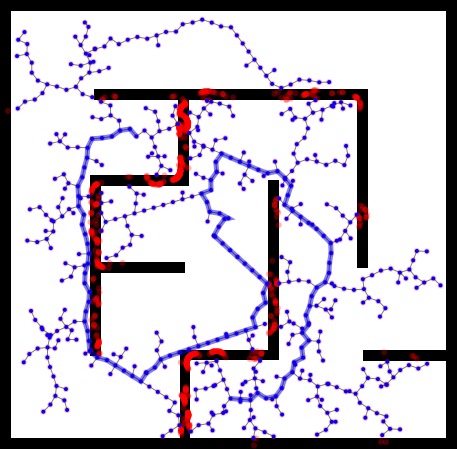
\includegraphics[width=\textwidth]{figs/compare-2d-rrtc1-rrtextcon-r1-s1.png}
\caption{RRT Ext-Con, R=1}
\end{subfigure}%
\quad
\begin{subfigure}[b]{0.3\textwidth}
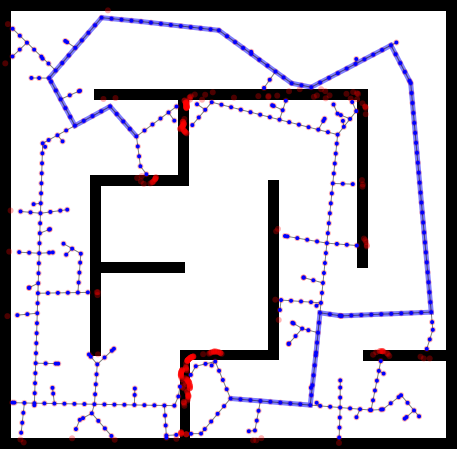
\includegraphics[width=\textwidth]{figs/compare-2d-rrtc1-rrtconcon-r1-s1.png}
\caption{RRT Con-Con, R=1}
\end{subfigure}%
\quad
\begin{subfigure}[b]{0.3\textwidth}
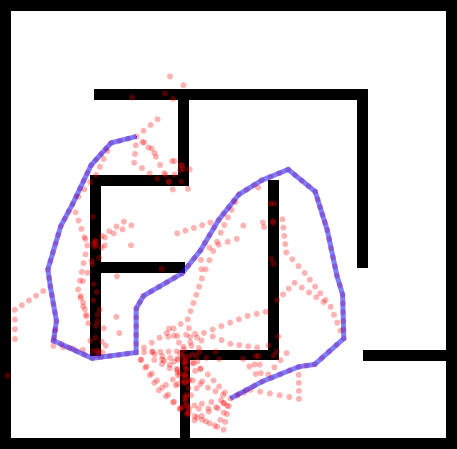
\includegraphics[width=\textwidth]{figs/compare-2d-rrtc1-checkmask-l00-s1.png}
\caption{Greedy PRM, $\lambda=0$}
\end{subfigure}%
\vspace{0.05in}
\begin{subfigure}[b]{0.3\textwidth}
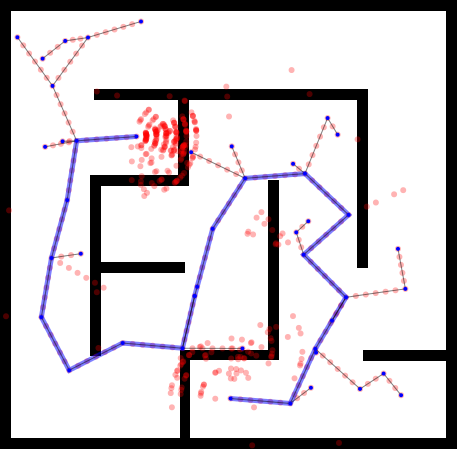
\includegraphics[width=\textwidth]{figs/compare-2d-rrtc1-rrtextcon-r6-s1.png}
\caption{RRT Ext-Con, R=6}
\end{subfigure}%
\quad
\begin{subfigure}[b]{0.3\textwidth}
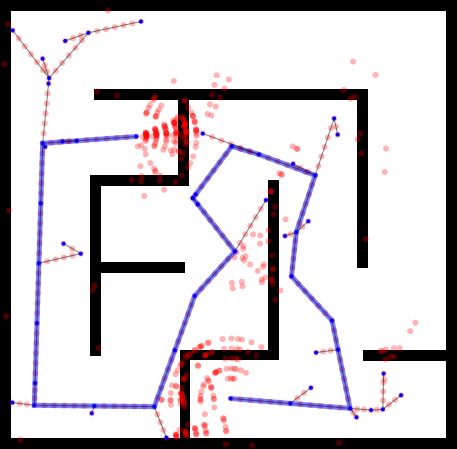
\includegraphics[width=\textwidth]{figs/compare-2d-rrtc1-rrtconcon-r6-s1.png}
\caption{RRT Con-Con, R=6}
\end{subfigure}%
\quad
\begin{subfigure}[b]{0.3\textwidth}
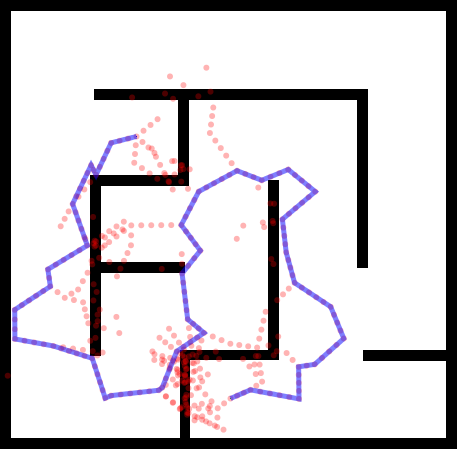
\includegraphics[width=\textwidth]{figs/compare-2d-rrtc1-checkmask-l10-s1.png}
\caption{Greedy PRM, $\lambda=1$}
\end{subfigure}%
\caption{Example runs with different planners,
   with the same sequence of samples.
   Note that Greedy PRM $\lambda=0$ is equivalent to LazyPRM.
   Red dots show collision checks.}
\label{fig:compare-2d-rrtc1-vis}
\end{figure}

\begin{figure}
\centering
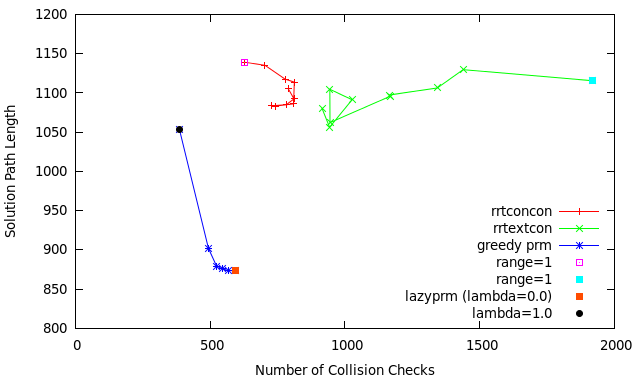
\includegraphics[width=0.8\textwidth]{figs/compare-2d-rrtc1-medians.png}
\caption{Plot of collision checks vs solution path cost for the
   different algorithms from the problem from
   Figure~\ref{fig:compare-2d-rrtc1-vis}.}
\end{figure}

\begin{figure}
\centering
\begin{subfigure}[b]{0.4\textwidth}
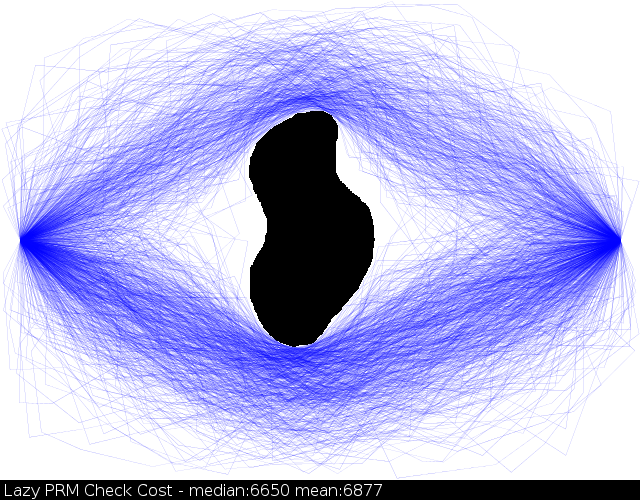
\includegraphics[width=\textwidth]{figs/timegreedy-bean-lambda-00.png}
\caption{Paths with $\lambda = 0$}
\end{subfigure}%
\quad
\begin{subfigure}[b]{0.4\textwidth}
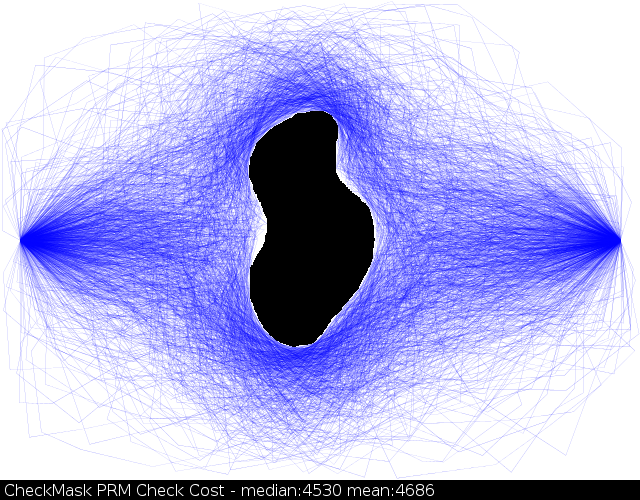
\includegraphics[width=\textwidth]{figs/timegreedy-bean-lambda-10.png}
\caption{Paths with $\lambda = 1$}
\end{subfigure}%
\caption{Examples of paths for a 2d problems
   for different values of $\lambda$.
   As $\lambda$ is increased,
   paths are longer, but are faster to find.}
\label{fig:bean}
\end{figure}

\begin{figure}
\centering
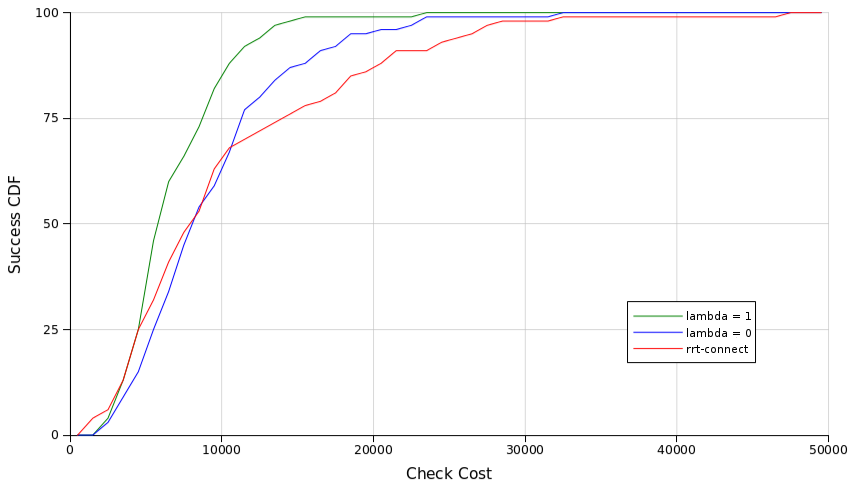
\includegraphics[width=0.8\textwidth]{figs/timegreedy-herbstep1-comparison-cdfs.png}
\caption{Comparison between different algorithms on a HERB problem.
   Must add in ESTs.}
\label{fig:herb-comparison-cdfs}
\end{figure}

\section{Repeated Queries}

For multiple queries within the same
$\mathcal{C}_{\mbox{\scriptsize free}}$,
the edge evaluations can be used in subsequent searches.
This ends up behaving similarily to E-graphs \cite{phillips2012egraphs}
with $\epsilon=1$
as described in Section~\ref{sec:egraphs},
with the exception that all evaluated edges are placed in the graph,
not just the edges on the solution path.
